
Jatkokoulutuksen FS-harjoitusohjelma (Formation Skydiving, kuviohyppy) sisältää 9 hyppyä ja niihin liittyvät tekniikat. Koulutusohjelman mukaan oppilaan tulee hypätä vähintään 5 ryhmähyppyä. Enemmänkin on mahdollista hypätä, jos hyppää FS-hyppyjä myös valinnaisilla suorituksilla. Ohjelmassa on tarkoitus siirtyä seuraavaan hyppyyn vasta, kun edellisen hypyn tavoite on saavutettu. Kaikki hypyt harjoitellaan maassa sekä pystyssä että laudoilla, jotta vapaapudotusaika tulisi käytettyä mahdollisimman tehokkaasti. 

\section{ Turvallisuus }
\label{fs-kuviohyppaaminen-turvallisuus}


FS-hyppäämisessä on monia huomioon otettavia turvallisuusasioita, koska mukana on useita hyppääjiä lähellä toisiaan. Koneessa hyppykaverin hyppyvarusteiden tarkkailu kuuluu asiaan. Uloshypyssä on katsottava tarkkaan mistä otteet otetaan, ettei ote ole vahingossa esimerkiksi varavarjon kahvasta. Uloshyppy on aina suunniteltava ja harjoiteltava lentokoneella tai uloshyppysimulaattorilla. Jos uloshyppy epäonnistuu, on kaikkien tiedettävä mitä silloin tehdään. Tästä pitää sopia etukäteen.  


Vapaapudotuksessa on vaarana, että joudutaan toisen hyppääjän ala- tai yläpuolelle. Törmäykset voivat joskus olla koviakin, ja sen vuoksi on aina käytettävä kovaa kypärää. Myöhemmässä vaiheessa myös tarkoitukselliset liikkeet voivat olla niin nopeita ja rajuja, että kovaa kypärää tarvitaan suojaamaan päätä esimerkiksi toisen jaloilta.  


Vastuu korkeuden tarkkailusta ja purkamisesta kuuluu kaikille. Oppilas-FS-hypyillä purkukorkeus on vähintään 1600 metriä, ja ainakin kahdella ensimmäisellä hypyllä 1800 metriä. Hypyn purkaminen oikeassa korkeudessa on oppilaan tehtävä. Purkumerkki näytetään selvästi, jonka jälkeen käännytään ja liu’utaan vapaaseen ilmatilaan. On tärkeää opetella hyvä, kantava liuku heti alusta lähtien, koska se vähentää törmäämisriskiä ja lisää näin turvallisuutta. Ylä- ja alapuolinen ilmatila täytyy tarkastaa ja näyttää avausmerkki aina ennen avausta. 


Hypättäessä muiden kanssa on aina oltava varautunut väistämään heti avauksen jälkeen (viedään kädet takimmaisille kantohihnoille heti varjon avautumisen jälkeen). Kun taivaalla on paljon ihmisiä samaan aikaan, on ohjauksen selkeys tärkeää; nopeat, yllättävät liikkeet saattavat haitata muiden lentämistä. 

\section{ Katsekontakti }
\label{fs-kuviohyppaaminen-katsekontakti}


FS-hyppäämisen tärkein perusasia on katse. Katse on ainoa keino kommunikoida ilmassa. 


Katsetta käyttäen säilytetään myös kiintopiste hyppykaverissa tai muodostelman keskipisteessä. Yleisin syy tasoeroihin ja vaakaetäisyyden syntymiseen on katsekontaktin puuttuminen, koska vartalo pyrkii liikkumaan katseen suuntaan. 

\section{ Perusasento  }
\label{fs-kuviohyppaaminen-perusasento}


Kaikki liikkeet aloitetaan perusasennosta, \textit{boxista}. (\ref{perusliikkeet-vapaassa-perusasento} s.\pageref{perusliikkeet-vapaassa-perusasento}) 

\section{ Liikkuminen vaakatasossa }
\label{fs-kuviohyppaaminen-liikkuminen-vaakatasossa}


Liikkuminen eteenpäin tapahtuu ojentamalla jalkoja suoremmiksi. Liikettä voi tehostaa siirtämällä samanaikaisesti käsiä kyynärpäistä taaksepäin. 


\begin{Figure}\centering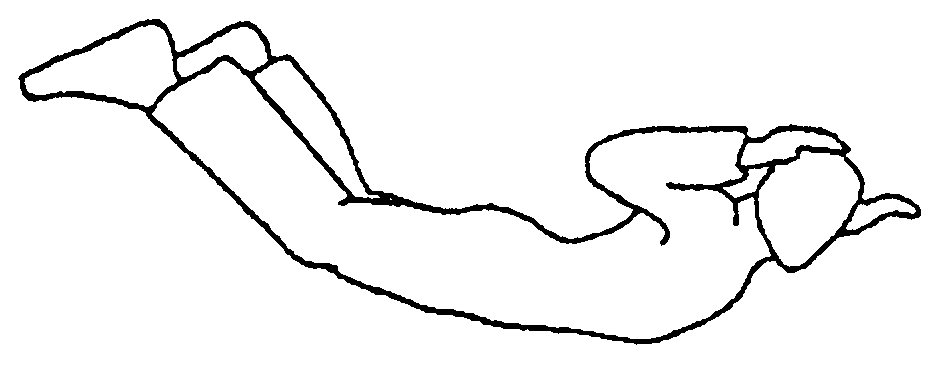
\includegraphics[width=0.7\textwidth]{Asento-liikeeteen.png}\captionof{figure}{Liikkuminen eteen}\end{Figure} 


Liikkuminen taaksepäin tapahtuu työntämällä käsiä eteenpäin ja koukistamalla samanaikaisesti polvia. 


\begin{Figure}\centering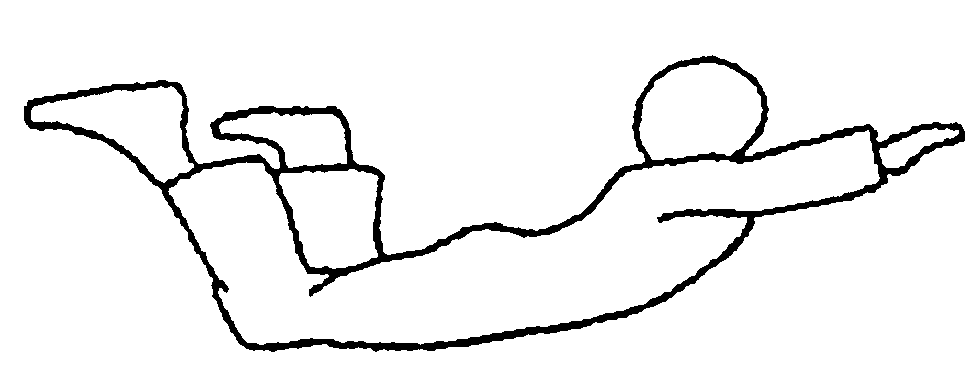
\includegraphics[width=0.7\textwidth]{Asento-liiketaakse.png}\captionof{figure}{Liikkuminen taakse}\end{Figure} 

\section{ Liikkuminen alas- ja ylöspäin }
\label{fs-kuviohyppaaminen-liikkuminen-alas-ja-ylospain}


Alas- ja ylöspäin liikkumista käytetään hyppykaverin kanssa samalla tasolla pysymiseen. Katsekontakti pariin täytyy säilyttää koko ajan. Pystysuoraan liikkumiseen käytetään taivutuksen lisäämistä (alaspäin suuntautuva liike) tai negatiivista taivutusta (ylöspäin suuntautuva liike, kupitus). 


\begin{Figure}\centering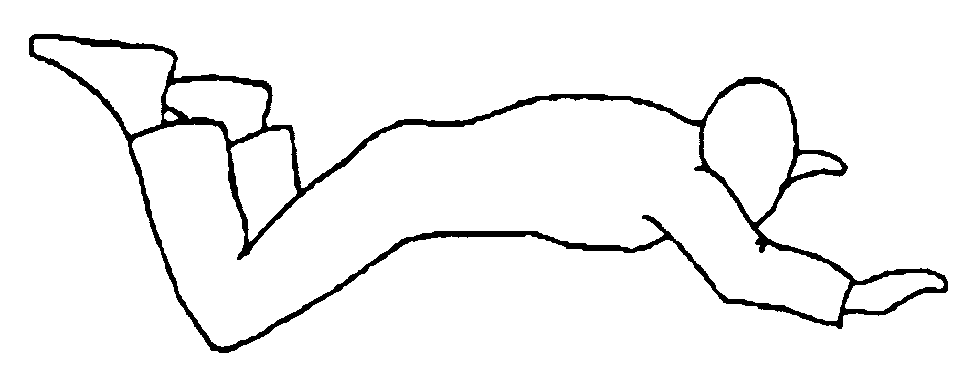
\includegraphics[width=0.7\textwidth]{Asento-liikeylos.png}\captionof{figure}{Liikkuminen ylös}\end{Figure} \begin{Figure}\centering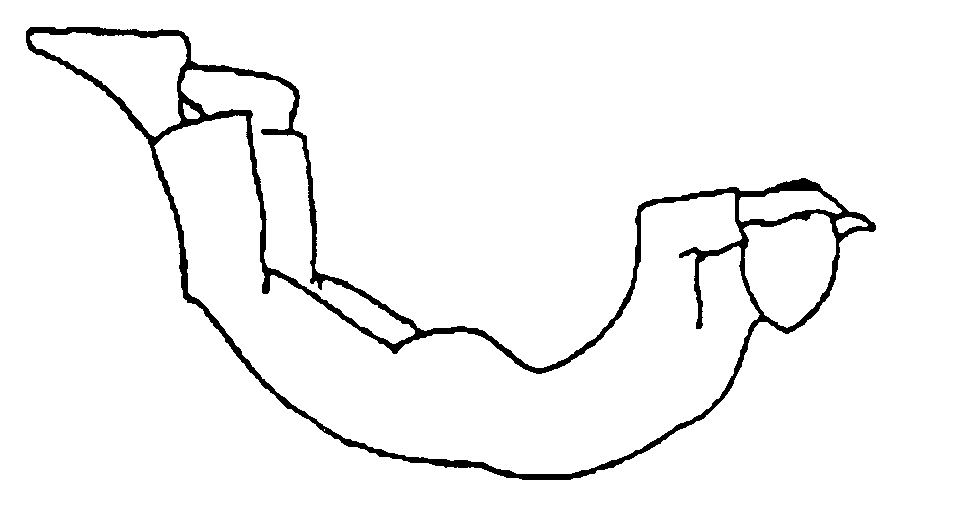
\includegraphics[width=0.7\textwidth]{Asento-liikealas.png}\captionof{figure}{Liikkuminen alas}\end{Figure} 

\section{ Käännökset }
\label{fs-kuviohyppaaminen-kaannokset}


Paikallaan pysyvä käännös perustuu käsien ja jalkojen samanaikaisiin liikkeisiin; keskivartalo pysyy suorassa linjassa koko käännöksen ajan. Käännös tehdään painamalla toisen puolen kättä ja vastakkaisen puolen jalkaa alaspäin. Käännöksen pysäyttäminen vaatii käsien ja jalkojen nopean ja terävän vastaliikkeen ja sen jälkeen asennon palautuksen perusasentoon. Käyttämällä enemmän käsiä kuin jalkoja saadaan aikaiseksi käännös polvien ympäri. Käyttämällä enemmän jalkoja kuin käsiä saadaan aikaan käännös ylävartalon ympäri. 

\section{ Liikkuminen sivuttain }
\label{fs-kuviohyppaaminen-liikkuminen-sivuttain}


Sivuttaisliikkeen aikaansaamiseksi kallistetaan vartaloa liikkeen suuntaan. Liikkeen pysäyttäminen vaatii vastaliikkeen eli kallistuksen toiseen suuntaan ennen perusasennon palauttamista. 

\section{ Otteiden ottaminen ja kuviossa lentäminen }
\label{fs-kuviohyppaaminen-otteiden-ottaminen-ja-kuviossa-lentaminen}


Otteita otettaessa on aina oltava samalla tasolla sen kanssa, josta otteita otetaan. Otteet otetaan joko ranteista tai gripeistä. Otteen on oltava napakka, mutta siinä ei saa olla vetoa. Ote on muodostelman viimeistelyä/kasaamista, eli hetkellinen pysäytys ennen muodostelman purkua, josta jatketaan seuraavaan muodostelmaan. Otteessa ei roikuta, vaan lennetään aktiivisesti omaa paikkaa ja ollaan valmiina siirtymään seuraavaan muodostelmaan. 

\section{ Hyppyohjelma }
\label{fs-kuviohyppaaminen-hyppyohjelma}


FS-harjoitusohjelma sisältää yhdeksän hyppyä ja niihin liittyvät tekniikat. Kouluttaja valitsee ohjelman hypyistä kyseiseen koulutusvaiheeseen sopivimman. 

\subsection{ Hyppy 1: Liikkuminen eteenpäin }
\label{fs-kuviohyppaaminen-hyppy-1-liikkuminen-eteenpain}


Uloshypyn jälkeen rentoudutaan, otetaan perusasento ja käännytään paria kohti. Lennetään eteenpäin parin luo, otetaan ranneotteet ja perusasento sekä tarkastetaan korkeus. Lennetään kuviossa oikein. Kun pari antaa merkin, päästetään otteet. Pari odottaa 2 sekuntia ja liikkuu muutaman metrin taaksepäin. Toistetaan liike eteenpäin. 


\begin{figure*}[]\centering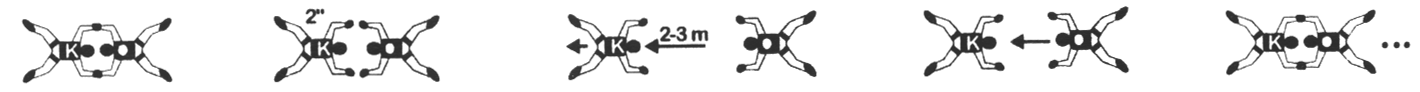
\includegraphics[width=0.7\textwidth]{FS-1.png}\caption{FS-hyppy 1}\end{figure*} 

\subsection{ Hyppy 2: Liikkuminen eteen- ja taaksepäin }
\label{fs-kuviohyppaaminen-hyppy-2-liikkuminen-eteen-ja-taaksepain}


Uloshypyn jälkeen rentoudutaan, otetaan perusasento ja käännytään paria kohti. Lennetään parin luo ja otetaan ranneotteet ja perusasento. Lennetään kuviossa oikein. Tarkastetaan korkeus ja päästetään otteet kun vetoa ei ole. Odotetaan 2 sekuntia ja liikutaan muutama metri taaksepäin. Toistetaan eteen – taakse -liikettä. 


\begin{figure*}[]\centering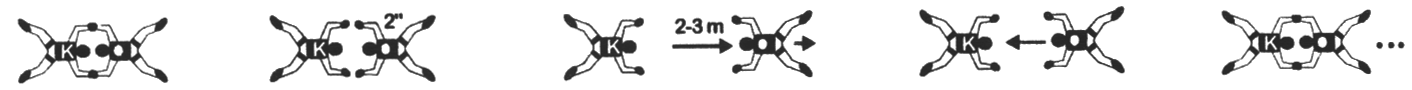
\includegraphics[width=0.7\textwidth]{FS-2.png}\caption{FS-hyppy 2}\end{figure*} 

\subsection{ Hyppy 3: Liikkuminen ylös- ja alaspäin }
\label{fs-kuviohyppaaminen-hyppy-3-liikkuminen-ylos-ja-alaspain}


Lennetään parin luo ja otetaan otteet. Tarkastetaan korkeus ja lennetään kuviossa oikein. Pari antaa merkin otteiden irrottamiseksi, kupittaa ja liikkuu ylöspäin metrin. Vähennetään taivutusta, kupitetaan metri ylöspäin parin tasalle ja otetaan perusasento. Pari taivuttaa ja liikkuu metrin alaspäin. Lisätään taivutusta, jotta päästään parin tasalle ja otetaan perusasento. Hypyllä ei oteta enää otteita. Pari pitää etäisyyden hypyn aikana muutamassa metrissä, jotta voidaan kupitettaessa kääntää päätä alaspäin ja silti pitää katsekontakti pariin. Pidetään asento koko ajan symmetrisenä. Toistetaan liikettä. 


\begin{figure*}[]\centering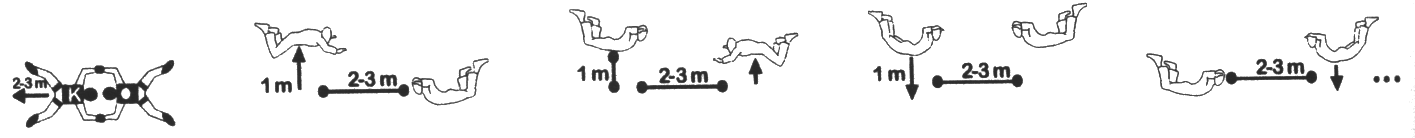
\includegraphics[width=0.7\textwidth]{FS-3.png}\caption{FS-hyppy 3}\end{figure*} 

\subsection{ Hyppy 4: Pystysuora liikkuminen yhdistettynä eteenpäin liikkeeseen }
\label{fs-kuviohyppaaminen-hyppy-4-pystysuora-liikkuminen-yhdistettyna-eteenpain-liikkeeseen}


Lennetään parin luo ja otetaan otteet. Pari peruuttaa pari metriä ja kupittaa ylöspäin metrin. Kupitetaan, lennetään eteenpäin parin luo ja otetaan perusasento. Otetaan otteet ja lennetään kuviossa oikein. Pari peruuttaa pari metriä ja taivuttaa alaspäin metrin. Taivutetaan, lennetään eteenpäin parin luo ja otetaan perusasento. Otetaan otteet ja lennetään kuviossa oikein. Kun tehdään liike, niin pyritään aina ensin liikkumaan pystysuoraan samalle tasolle parin kanssa ja vasta sitten eteenpäin otetta varten. Pidetään katsekontakti pariin koko ajan. Toistetaan liikettä. 


\begin{figure*}[]\centering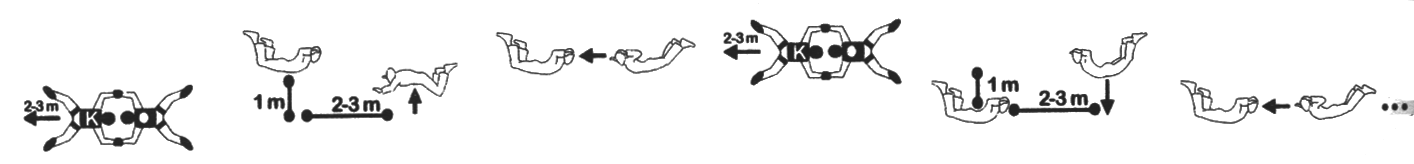
\includegraphics[width=0.7\textwidth]{FS-4.png}\caption{FS-hyppy 4}\end{figure*} 

\subsection{ Hyppy 5: 90° käännös }
\label{fs-kuviohyppaaminen-hyppy-5-90deg-kaannos}


Käännöksissä paria pidetään kiintopisteenä. Käännökset tehdään puolitähdestä avohaitariin ja siitä takaisin puolitähteen. Lennetään parin luo ja otetaan otteet. Pari antaa merkin, jonka jälkeen irrotetaan vasemman käden ote ja muodostelma avataan 90° puolitähdeksi. Kun otteessa ei ole vetoa, annetaan merkki. Päästettäessä ote odotetaan hetki ennen kuin aloitetaan liike. Käännytään 90° oikealle ja otetaan ote vasemmalla kädellä (avohaitariin). Annetaan merkki ja käännytään takaisin puolitähteen. Pidetään huoli, että otteita otettaessa ollaan samalla tasolla parin kanssa. Kuviosta toiseen liikuttaessa tehdään ensin oikea liike ja vasta sitten otetaan otteet. Kun otetaan ote, varmistetaan, että se on kevyt ja että lennetään paikalla eikä otteessa roikuta. Toistetaan liikettä. 


\begin{figure*}[]\centering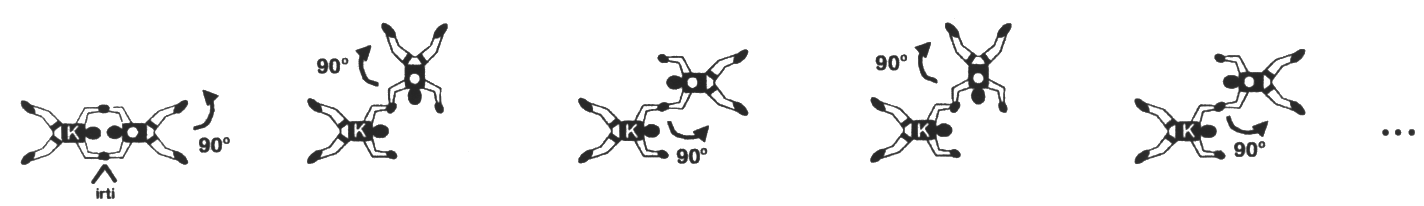
\includegraphics[width=0.7\textwidth]{FS-5.png}\caption{FS-hyppy 5}\end{figure*} 

\subsection{ Hyppy 6: 180° käännös }
\label{fs-kuviohyppaaminen-hyppy-6-180deg-kaannos}


Lennetään parin luo ja otetaan otteet. Käännytään 90° oikealle ja pysähdytään ilman otteita olevaan sidebody-muodostelmaan. Pidetään etäisyyttä ja kulmaa 2 sekuntia. Käännytään 180° vasemmalle vastakkaiseen sidebody-muodostelmaan pitäen paria kiintopisteenä. Pidetään etäisyyttä ja kulmaa 2 sekuntia. Pysähdytään käännösten välillä, jotta pystytään keskittymään ja jotta käännökset eivät alkaisi mennä yli halutun astemäärän. Jos ajaudutaan sivuttain poispäin parista, niin käännytään välittömästi paria kohti ja jatketaan käännöksiä toiseen suuntaan. Toistetaan liikettä. 


\begin{figure*}[]\centering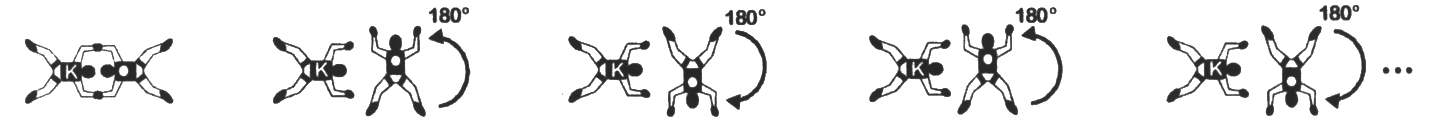
\includegraphics[width=0.7\textwidth]{FS-6.png}\caption{FS-hyppy 6}\end{figure*} 

\subsection{ Hyppy 7: 360° käännös }
\label{fs-kuviohyppaaminen-hyppy-7-360deg-kaannos}


Lennetään parin luo ja otetaan otteet. Parin annettua merkin käännytään 360° oikealle. Käytetään jalkoja käännökseen. Muistetaan perusasennon symmetrisyys, aloitus – lähestyminen – pysäytys ja otetaan otteet. Käännytään 360° vasemmalle. Ollaan kärsivällisiä ja odotetaan ennen käännöksen aloittamista, että kuvio on purettu ja että parin kanssa lennetään vierekkäin samalla tasolla. Muistetaan, että liike tulee hidastaa hyvissä ajoin, jottei kääntyminen mene yli halutun astemäärän. Toistetaan liikettä. 


\begin{figure*}[]\centering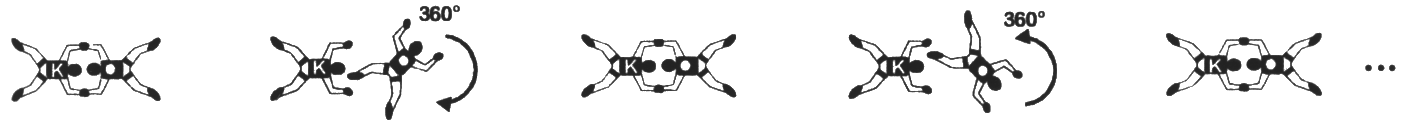
\includegraphics[width=0.7\textwidth]{FS-7.png}\caption{FS-hyppy 7}\end{figure*} 

\subsection{ Hyppy 8: Liikkuminen sivuttain }
\label{fs-kuviohyppaaminen-hyppy-8-liikkuminen-sivuttain}


Liike tehdään parin edessä aloittaen tähdestä ja liikkuen siitä sivuttain avohaitariin, jonka jälkeen toisen puolen avohaitariin ja taas takaisin tähteen. Lennetään parin luo ja otetaan otteet. Liikutaan oikealle vartalonmitan verran, pysäytetään ja otetaan ote. Liikutaan vasemmalle kahden vartalonmitan verran, pysäytetään ja otetaan ote. Toistetaan liikettä. 


\begin{figure*}[]\centering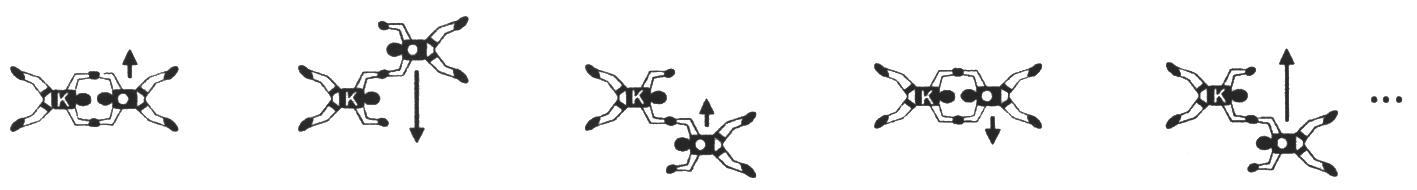
\includegraphics[width=0.7\textwidth]{FS-8.png}\caption{FS-hyppy 8}\end{figure*} 

\subsection{ Hyppy 9: Lähestyminen sivuttain }
\label{fs-kuviohyppaaminen-hyppy-9-lahestyminen-sivuttain}


Liike tehdään parin edessä aloittaen tähdestä ja tehden 90° käännös oikealle ja sen jälkeen liikkuen sivulle paria kohden, jotta hän saa otteet. Tämän jälkeen pari antaa merkin ja irrottaa otteet. Lennetään parin luo ja otetaan otteet. Käännytään vasemmalle 90° ja liikutaan sivuttain parin luo. Pari antaa merkin ja irrottaa otteet. Muistetaan käyttää koko vartaloa sivuttain liikkeessä. Pyritään tekemään käännökset aina rauhallisesti, jotta ei käännytä yli. Toistetaan liikettä. 


\begin{figure*}[]\centering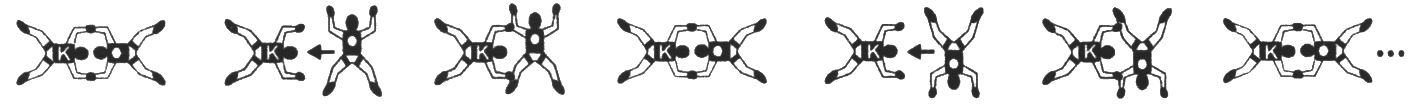
\includegraphics[width=0.7\textwidth]{FS-9.png}\caption{FS-hyppy 9}\end{figure*} 

